\chapter{State of the Art}
\graphicspath{{state-of-the-art/figures/}}

In recent years, the remarkable advancements in Natural Language Processing (NLP) have been primarily driven by the development of LLMs. These LLMs, such as GPT (Generative Pretrained Transformer)\cite{openai:gpt} and BERT (Bidirectional Encoder Representations from Transformers)\cite{devlin2019bert}, have demonstrated remarkable capabilities in understanding and generating human-like text. However, despite their impressive performance, LLMs still face challenges in effectively retrieving and incorporating relevant context for generating accurate and coherent responses.

Enter RAG systems, a novel approach that seeks to overcome the limitations of traditional LLMs by integrating retrieval mechanisms with generation models. RAG systems combine the strengths of both retrieval and generation techniques to enhance the quality and relevance of generated text.

This chapter provides a comprehensive exploration of RAG systems, delving into their architecture, components, training processes, applications, advantages, and challenges. We begin by establishing a foundational understanding of LLMs and their evolution, laying the groundwork for understanding the need for RAG systems. We then proceed to dissect the intricacies of RAG systems, discussing the role of retrieval in providing context and the role of generation in producing fluent responses.

Through detailed examination and analysis, we uncover the inner workings of RAG systems, exploring how retrieval and generation components interact within the architecture. Real-world applications and use cases of RAG systems across various domains are elucidated, demonstrating their potential to revolutionize tasks such as question answering, dialogue generation, and content creation.

Furthermore, we evaluate the advantages and limitations of RAG systems compared to traditional LLMs and other approaches in NLP. By examining performance metrics, challenges, and future directions, we gain insights into the transformative impact of RAG systems on the field of natural language processing.

In summary, this chapter serves as a comprehensive guide to RAG systems, offering readers a deep dive into one of the most promising advancements in NLP. As we navigate through the complexities and potentials of RAG systems, we pave the way for understanding their role in shaping the future of human-computer interaction and language understanding.

\section{Machine Learning}

\subsection{Definition}


Machine Learning, often abbreviated as ML, is a subset of artificial intelligence (AI) that focuses on the development of computer algorithms that improve automatically through experience and by the use of data. In simpler terms, machine learning enables computers to learn from data and make decisions or predictions without being explicitly programmed to do so \cite{datacamp:ml}.

At its core, machine learning is all about creating and implementing algorithms that facilitate these decisions and predictions. These algorithms are designed to improve their performance over time, becoming more accurate and effective as they process more data.

In traditional programming, a computer follows a set of predefined instructions to perform a task. However, in machine learning, the computer is given a set of examples (data) and a task to perform, but it's up to the computer to figure out how to accomplish the task based on the examples it's given.

For instance, if we want a computer to recognize images of cats, we don't provide it with specific instructions on what a cat looks like. Instead, we give it thousands of images of cats and let the machine learning algorithm figure out the common patterns and features that define a cat. Over time, as the algorithm processes more images, it gets better at recognizing cats, even when presented with images it has never seen before.

This ability to learn from data and improve over time makes machine learning incredibly powerful and versatile. It's the driving force behind many of the technological advancements we see today, from voice assistants and recommendation systems to self-driving cars and predictive analytics.

\subsection{Relationships to other fields}

Artificial Intelligence (AI) encompasses the field of computer science dedicated to creating systems capable of emulating human-like intelligence, problem-solving, and decision-making. Machine Learning (ML) is a subset of AI focused on enabling computers to learn from data without being explicitly programmed. Within ML, Deep Learning stands out as a subfield that employs neural networks with multiple layers to learn complex representations of data, particularly effective in tasks like image and speech recognition. ML and Deep Learning are integral components of AI, providing the framework for developing intelligent systems capable of learning, reasoning, and adapting to new information, thereby advancing the capabilities of AI across various domains.

\begin{figure}[htpb]
    \centering
    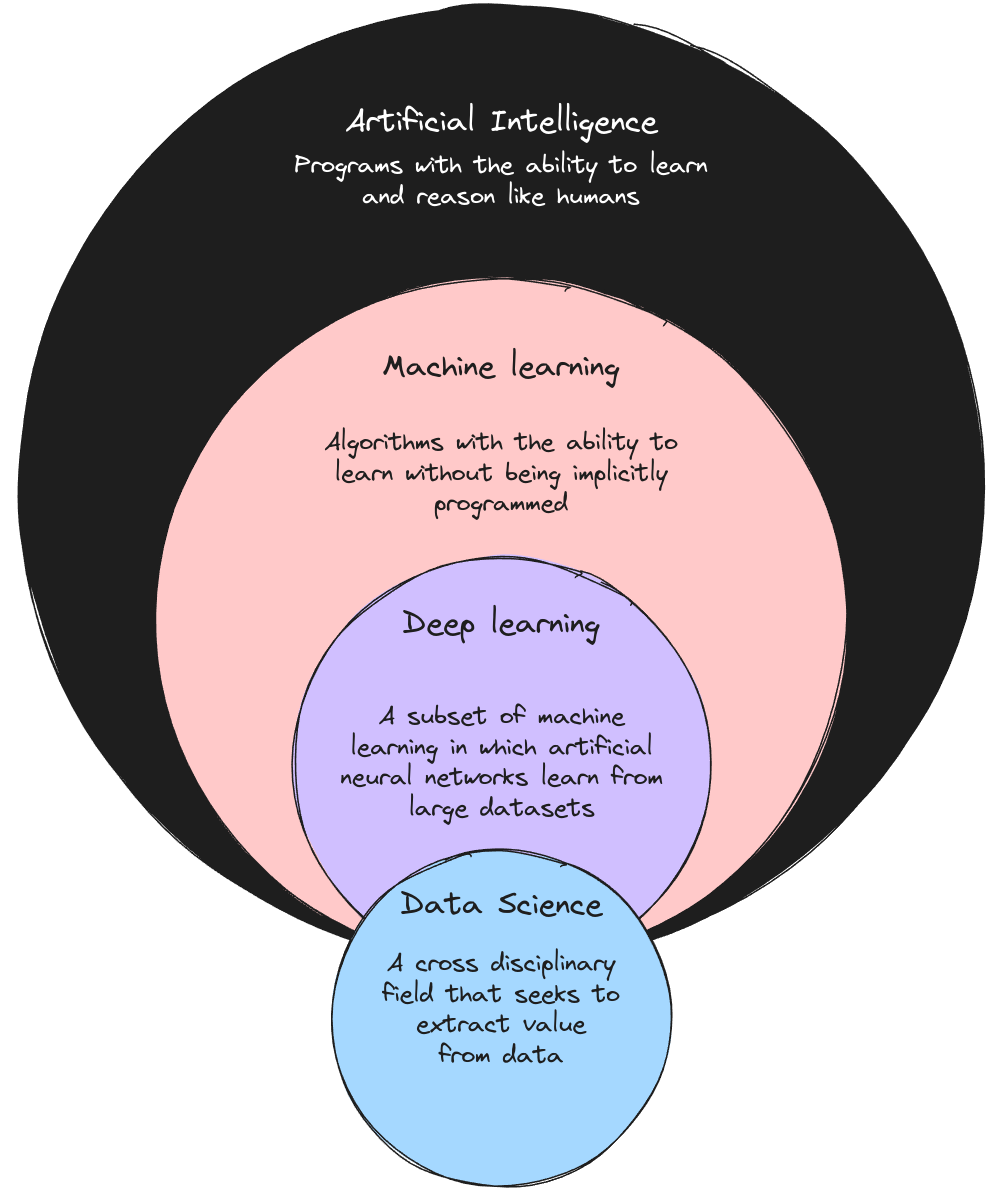
\includegraphics[width=\textwidth,height=6cm,keepaspectratio=true]{ml.png}
    \caption{
        \it{Machine learning as subfield of AI \cite{datacamp:ml}.}
    }
\end{figure}

\subsection{Types of Machine Learning}

Machine Learning can be broadly categorized into several types based on the learning approach, the availability of labeled data, and the feedback mechanism. The main types of machine learning are:

\begin{figure}[htpb]
    \centering
    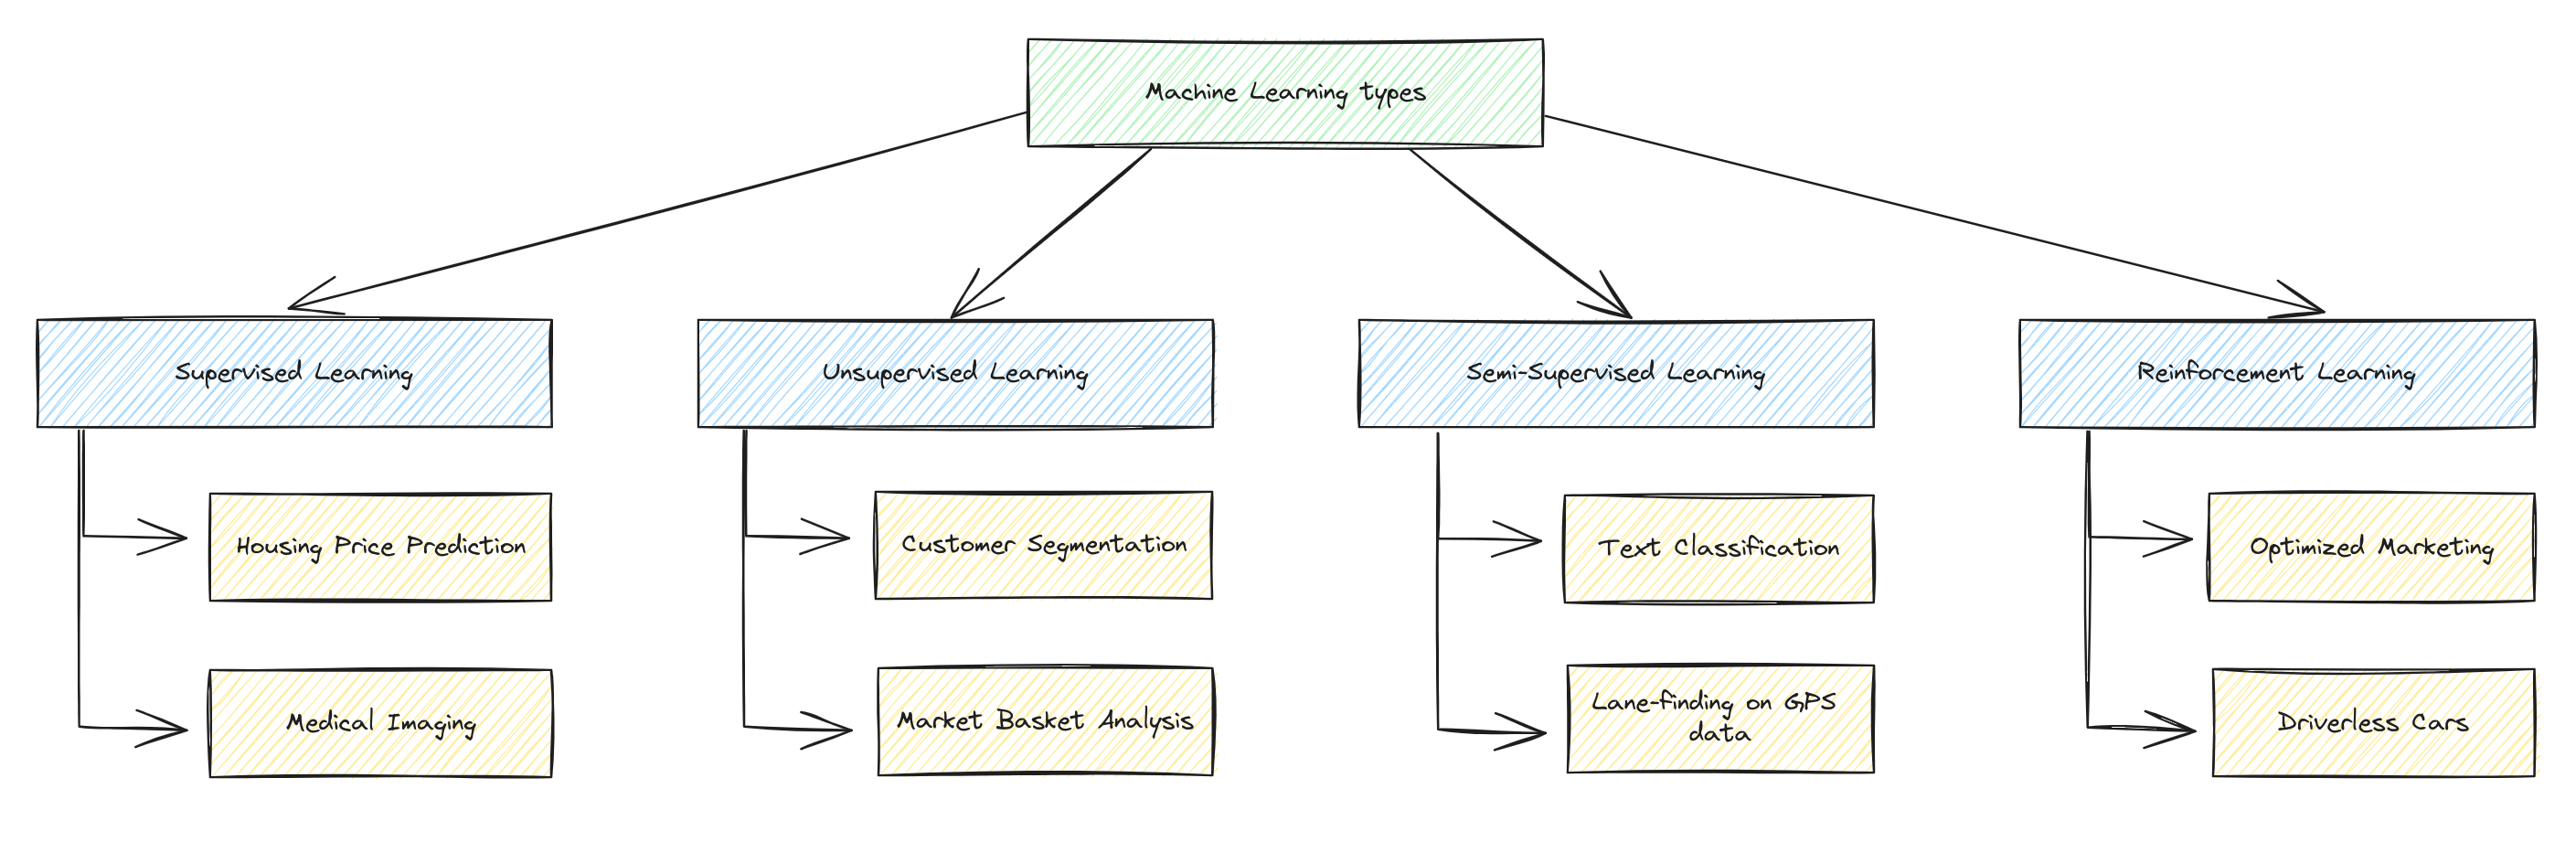
\includegraphics[width=\textwidth,height=6cm,keepaspectratio=true]{ml-types.png}
    \caption{
        \it{Types of machine Learning.}
    }
\end{figure}

\subsubsection*{Supervised Learning}
Supervised machine learning learns patterns and relationships between input and output data. It is defined by its use of labeled data. A labeled data is a dataset that contains a lot of examples of Features and Target. Supervised learning uses algorithms that learn the relationship of Features and Target from the dataset. This process is referred to as Training or Fitting \cite{datacampsupervised}.


\subsubsection*{Unsupervised Learning:}

Unsupervised learning, also known as unsupervised machine learning, uses machine learning algorithms to analyze and cluster unlabeled data sets. These algorithms discover hidden patterns or data groupings without the need for human intervention. Unsupervised learning models are utilized for three main tasks—clustering, association, and dimensionality reduction \cite{ibmunsupervised}.

\subsubsection*{Semi-Supervised Learning:}

Semi-supervised learning is a relatively new and less popular type of machine learning that, during training, blends a sizable amount of unlabeled data with a small amount of labeled data. Semi-supervised learning is between supervised learning (with labeled training data) and unsupervised learning (unlabeled training data).

Semi-supervised learning offers a lot of real-world applications. There is a dearth of labeled data in many fields. Because they involve human annotators, specialized equipment, or expensive, time-consuming studies, the labels (target variable) could be challenging to get \cite{datacampsupervised}.


\subsubsection*{Reinforcement Learning:}

Reinforcement learning (RL) is a machine learning technique that trains software to make decisions to achieve the most optimal results. It mimics the trial-and-error learning process that humans use to achieve their goals \cite{awsrl}.

\subsection{Limitations of Machine Learning: Challenges and Considerations}

Although machine learning is a powerful technique for extracting knowledge from data, it also has certain limitations that are important to consider:

\begin{itemize}
    \item{\textbf{Data dependency:} Machine learning heavily relies on the quality and quantity of training data. If the data is poorly labeled or unrepresentative, it can lead to errors in predictions.}
    \item{\textbf{Overfitting:} When the model is too complex compared to the training data, it can overfit and not generalize well to test data. This can also result in poor performance for new data.}
    \item{\textbf{Explainability:} Machine learning models can be very complex and difficult to understand. It can be challenging to understand how the model makes decisions and to explain these decisions to users.}
    \item{\textbf{Biased data:} Training data can be biased due to factors such as data selection, human biases, or measurement errors. This can lead to biased predictions for test data.}
    \item{\textbf{Lack of diversity:} Machine learning models may lack diversity in the types of data they can handle. For example, machine learning models may struggle to process unstructured data such as images, sounds, and texts.}
    \item{\textbf{Computational cost:} Machine learning algorithms may require high computational power and significant storage resources to process large amounts of data. This can be costly and time-consuming to train and implement models.}
\end{itemize}

\section{Deep Learning}

\subsection{Definition}

Deep learning is a type of machine learning that teaches computers to perform tasks by learning from examples, much like humans do. Imagine teaching a computer to recognize cats: instead of telling it to look for whiskers, ears, and a tail, you show it thousands of pictures of cats. The computer finds the common patterns all by itself and learns how to identify a cat. This is the essence of deep learning.

In technical terms, deep learning uses something called "neural networks," which are inspired by the human brain. These networks consist of layers of interconnected nodes that process information. The more layers, the "deeper" the network, allowing it to learn more complex features and perform more sophisticated tasks \cite{datacamp:dl}.


\subsection{Deep Learning vs. Machine Learning}

Deep learning stands apart from traditional machine learning in its approach to data and learning methods.
Machine learning algorithms typically rely on structured, labeled data for predictions, where specific features are defined and organized into tables.
While machine learning can handle unstructured data, it often requires preprocessing to structure it. In contrast, deep learning streamlines this process by directly processing unstructured data such as text and images. It automates feature extraction, reducing reliance on human experts. For instance, in categorizing pet photos, deep learning algorithms autonomously identify key features, like ears, crucial for distinguishing between animals. In contrast, machine learning requires manual feature hierarchy establishment by human experts.

\subsection{Deep Learning Applications}

Deep learning has a wide range of applications across various domains due to its ability to learn complex patterns from large volumes of data. Some of the different types of applications for deep learning include:

\subsubsection*{Image Recognition and Computer Vision:}

\begin{itemize}
    \item Deep learning is extensively used for tasks such as image classification, object detection, facial recognition, and image segmentation.
    \item Applications include self-driving cars, medical image analysis, surveillance systems, and augmented reality.
\end{itemize}

\subsubsection*{Natural Language Processing (NLP):}

\begin{itemize}
    \item Deep learning is employed for understanding and generating human language, enabling tasks such as sentiment analysis, machine translation, text summarization, and chatbots.
    \item Applications include virtual assistants, language translation services, social media sentiment analysis, and customer support chatbots.
\end{itemize}


These are just a few examples of the diverse applications of deep learning, demonstrating its versatility and impact across various industries and fields.

\clearpage

\section{Natural Language Processing (NLP)}

Natural Language Processing (NLP) serves as a crucial technology within artificial intelligence, facilitating communication between humans and computers. It represents a multidisciplinary field empowering machines to comprehend, analyze, and produce human language, thus facilitating seamless human-machine interaction. The importance of NLP manifests in its diverse applications, spanning automated customer support to instantaneous language translation, showcasing its pivotal role in modern computing.

\subsection{What is Natural Language Processing?}

Natural Language Processing (NLP) is a sub-discipline of computer science providing a bridge between natural languages and computers. It helps empower machines to understand, process, and analyze human language. NLP's significance as a tool aiding comprehension of human-generated data is a logical consequence of the context-dependency of data. Data becomes more meaningful through a deeper understanding of its context, which in turn facilitates text analysis and mining. NLP enables this with the communication structures and patterns of humans \cite{torfi2021natural}.

NLP encompasses the task of enabling machines to comprehend, interpret, and generate human language in a manner that is not only valuable but also meaningful. OpenAI\footnote{\url{https://openai.com/}}, renowned for pioneering sophisticated language models such as ChatGPT\footnote{\url{https://chat.openai.com}}, underscores the significance of NLP in fostering the development of intelligent systems capable of comprehending, responding to, and generating text. This advancement in technology serves to enhance user-friendliness and accessibility across various applications.

\subsection{How Does NLP Work?}

NLP is a fascinating field that delves into the intricate mechanisms underlying human language comprehension and generation by machines. This section aims to unravel the complexities of NLP, shedding light on the fundamental principles and techniques that drive its functionality. By exploring the inner workings of NLP, we gain insight into how machines process and analyze natural language data, paving the way for groundbreaking applications in artificial intelligence and human-computer interaction. Through this exploration, we embark on a journey to discover the algorithms, models, and methodologies that empower machines to navigate the vast landscape of human language with precision and sophistication.

\subsubsection*{Components of NLP}

Natural Language Processing is not a monolithic, singular approach, but rather, it is composed of several components, each contributing to the overall understanding of language. The main components that NLP strives to understand are Syntax, Semantics, Pragmatics, and Discourse.

\begin{itemize}
    \item \textbf{Syntax:} Syntax pertains to the arrangement of words and phrases to create well-structured sentences in a language.
    \item \textbf{Semantics:} Semantics is concerned with understanding the meaning of words and how they create meaning when combined in sentences.
    \item \textbf{Pragmatics:} Pragmatics deals with understanding language in various contexts, ensuring that the intended meaning is derived based on the situation, speaker's intent, and shared knowledge.
    \item \textbf{Discourse:} Discourse focuses on the analysis and interpretation of language beyond the sentence level, considering how sentences relate to each other in texts and conversations.
\end{itemize}

\subsubsection*{NLP techniques and methods}

NLP employs a diverse array of techniques and methodologies to analyze and comprehend human language. Below are some foundational techniques utilized in NLP:

\begin{itemize}
    \item \textbf{Tokenization:} This process involves segmenting text into individual units, such as words, phrases, or symbols, known as tokens.
    \item \textbf{Parsing:} Parsing entails examining the grammatical structure of a sentence to extract its meaning and syntactic relationships.
    \item \textbf{Lemmatization:} This technique involves reducing words to their base or root form, facilitating the grouping of different word forms with the same meaning.
    \item \textbf{Named Entity Recognition (NER):} NER is utilized to identify and classify entities within text, such as persons, organizations, locations, and other named items.
    \item \textbf{Sentiment Analysis:} This method enables the assessment of the sentiment or emotion expressed in a piece of text, aiding in understanding the underlying mood or opinion.
\end{itemize}

\subsubsection*{What is NLP Used For?}

With some of the basic concepts now defined, one can explore how natural language processing is applied in the modern world.

\begin{itemize}
    \item \textbf{Automatic Translation:} Automatic translation systems use NLP techniques to translate texts from one language to another.
    \item \textbf{Chatbots and Virtual Assistants:} Chatbots and virtual assistants use NLP to understand user's natural language and provide appropriate responses.
    \item \textbf{Automatic Summarization:} NLP algorithms can be employed to summarize lengthy documents into a few sentences.
    \item \textbf{Sentiment Analysis:} NLP is utilized to analyze sentiments expressed in text, which can be beneficial for businesses in assessing customer satisfaction.
    \item \textbf{Information Extraction:} NLP systems can extract important information such as names, locations, and dates from texts.
    \item \textbf{Speech Recognition:} Speech recognition systems utilize NLP techniques to convert speech into text.
    \item \textbf{Autocorrection:} NLP algorithms are utilized in autocorrection programs to suggest grammatical and spelling corrections.
    \item \textbf{Text Analysis:} NLP is used to analyze large volumes of text to detect trends, themes, and patterns.
    \item \textbf{Automatic Text Generation:} NLP enables the automatic generation of text for various applications, such as report writing or content creation.
\end{itemize}

\clearpage

\section{Neural networks}

Neural Networks (NNs) are computational models composed of layers of neurons that can learn from data \cite{oshea2015introduction}. They are versatile and robust models capable of learning directly from raw data, without the need for manually selected features \cite{lipton2015critical}. NNs employ a training algorithm known as backpropagation, which adjusts the model's parameters based on a loss function \cite{lipton2015critical}.

\subsection{Feedforward networks}

A feedforward neural network is characterized by its architecture, devoid of cycles, where the output of layer \(i\) can be computed using the outputs from layer \(i - 1\) \cite{lipton2015critical}. The architecture of a neural network encompasses its structure, including the number of hidden layers and neurons, as well as the functions employed for computations. These selections, known as hyperparameters, are parameters whose values are not determined by the learning algorithm \cite{nnanddl}. Figure \ref{fig:ffn} shows a typical feedforward network architecture.


\begin{figure}[H]
    \centering
    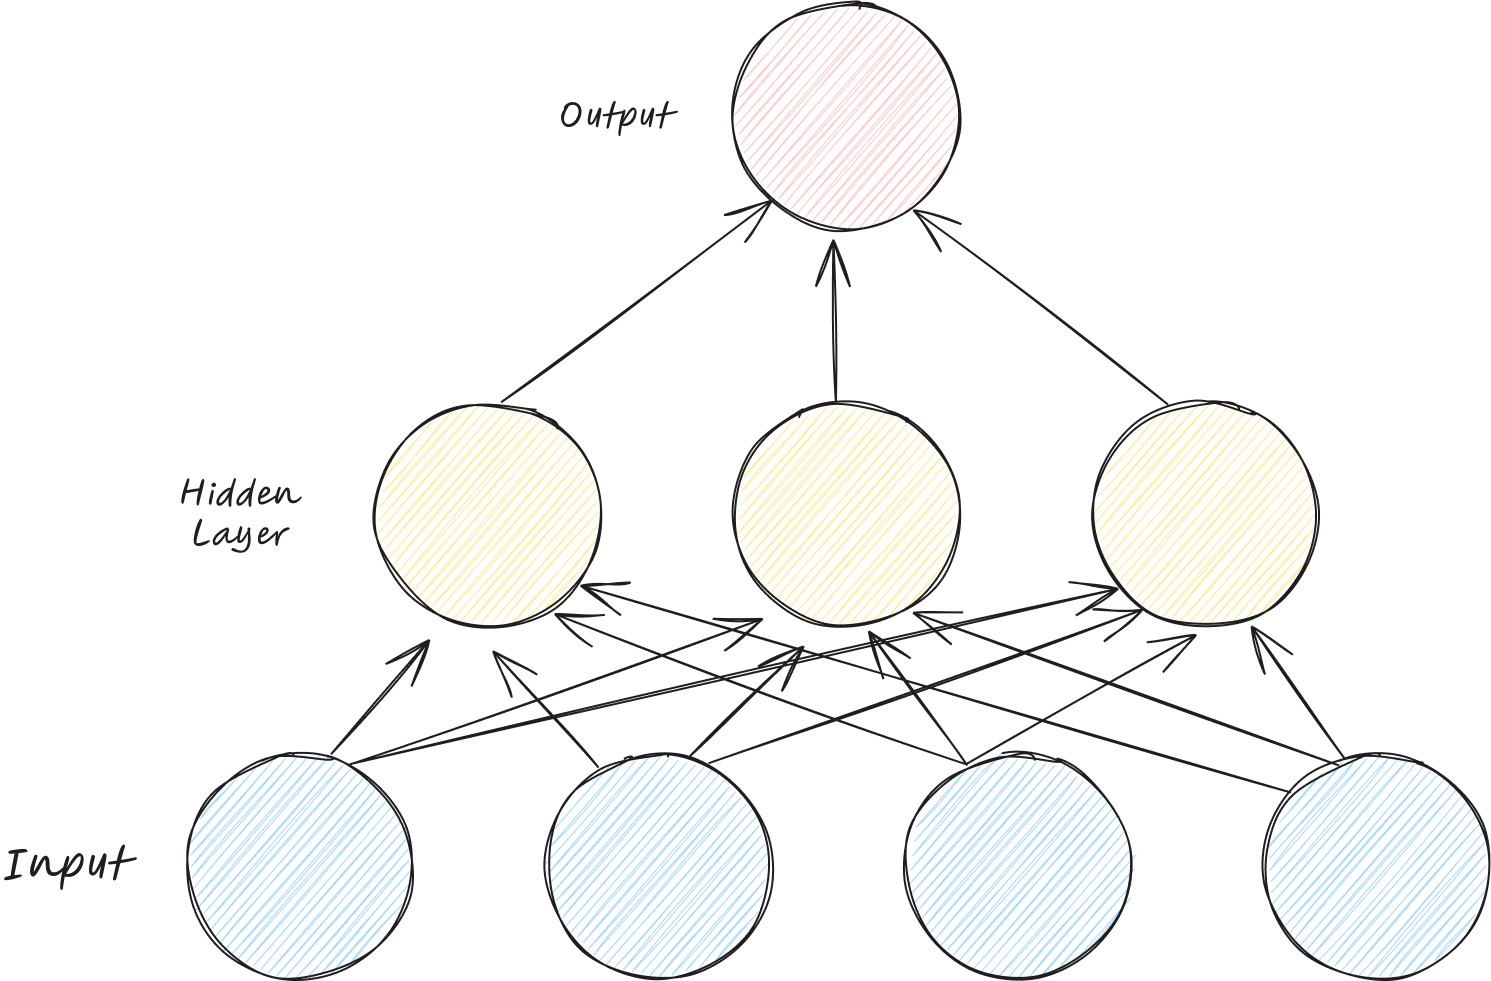
\includegraphics[width=\textwidth,height=6cm,keepaspectratio=true]{ffn.png}
    \caption{
        \it{Example of a feedforward neural network architecture. The network has an
            input layer with four neurons, one hidden layer with three neurons and an output layer with a single neuron \cite{lipton2015critical}.}
    }
    \label{fig:ffn}
\end{figure}

As depicted in Figure \ref{fig:ffn}, neural networks comprise an input layer, \(n\) hidden layers, and an output layer. The input layer receives the data that the network needs to process, which then traverses through the hidden layers before reaching the output layer. The output layer provides the model's result for the given input data. When a neural network contains multiple hidden layers, it qualifies as a deep neural network (DNN) and falls within the domain of deep learning \cite{oshea2015introduction}. Each layer consists of \(i\) neurons, with connections between each neuron in a layer and every neuron in the previous layer, except for the input layer.

Neurons serve as fundamental computational units and, as previously indicated, establish connections with all neurons in the preceding layer. Each connection is characterized by a numerical parameter referred to as a weight \cite{lipton2015critical}.


\begin{figure}[H]
    \centering
    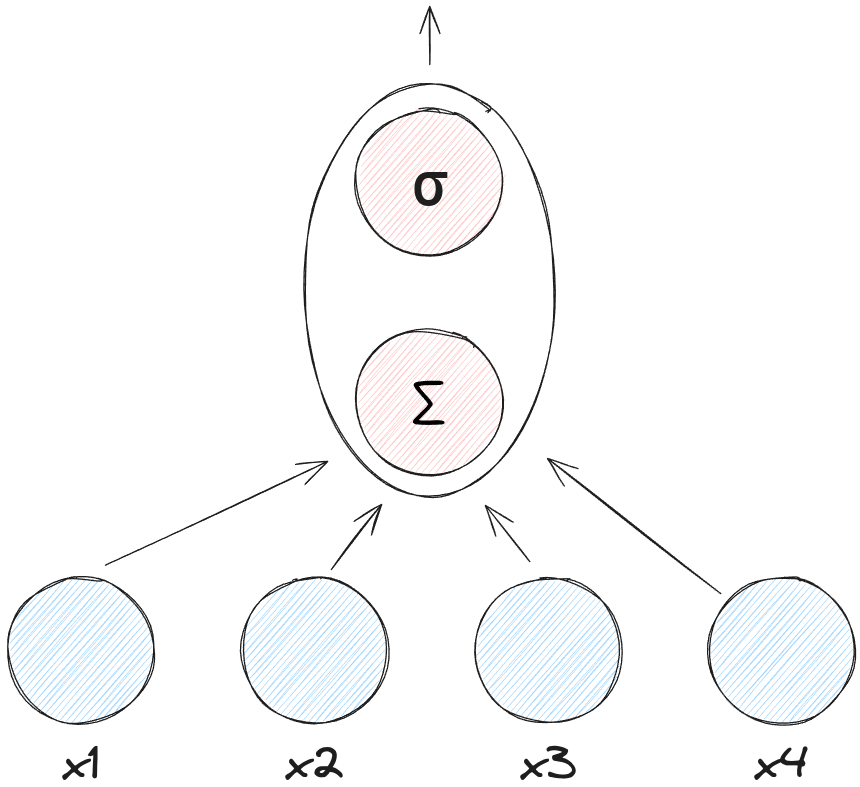
\includegraphics[width=\textwidth,height=6cm,keepaspectratio=true]{1nn.png}
    \caption{
        \it{Example of computation within a single neuron, where the weighted sum
            of inputs is passed through an activation function to get the output of the neuron \cite{lipton2015critical}.}
    }
    \label{fig:1nn}
\end{figure}

As show in Figure \ref{fig:1nn}, the neuron receives inputs from neurons of the preceding layer, denoted as \(x_1, x_2, ..., x_n\). Each neuron-to-neuron connection is assigned a weight, representing the strength of the connection. The output from a preceding neuron is multiplied by the weight of the connection and then summed for each connected neuron, yielding the weighted sum of values.

Although not visually represented in Figure \ref{fig:1nn}, a bias parameter is introduced to the weighted sum, thereby altering \(a_j\) to

\begin{equation}
    a_j = \sum_{j'} w_{jj'}x_{j'} + b
\end{equation}

The bias serves to adjust the neuron's output independently of the input. This capability enables the model to alter the neuron's output during the learning process without necessitating adjustments to the weights, thereby facilitating finer control \cite{nnanddl}.

The weighted sum is subsequently forwarded to an activation function, which determines the neuron's output or its degree of "activation." An illustration of such an activation function is the sigmoid function denoted as \(\sigma\), as depicted in Figure \ref{fig:1nn}. The mathematical expression for the sigmoid function is:

\begin{equation}
    \sigma(a_j) = \frac{1}{1+e^{-a_j}}
\end{equation}

According to Nielsen \cite{nnanddl}, two other common activation functions include \(\tanh \phi\),
which is defined as

\begin{equation}
    \phi(a_j) = \tanh(a_j) = \frac{e^{a_j} - e^{-a_j}}{e^{a_j} + e^{-a_j}}
\end{equation}

and Rectified Linear Unit (ReLU), which is defined by equation

\begin{equation}
    R(a_j) = max(0, a_j)
\end{equation}

Symbol \(a_j\) refers to the result of adding together the weighted sum and bias. The
outputs of these functions are visualized in Figure \ref{fig:activation}.


\begin{figure}[H]
    \centering
    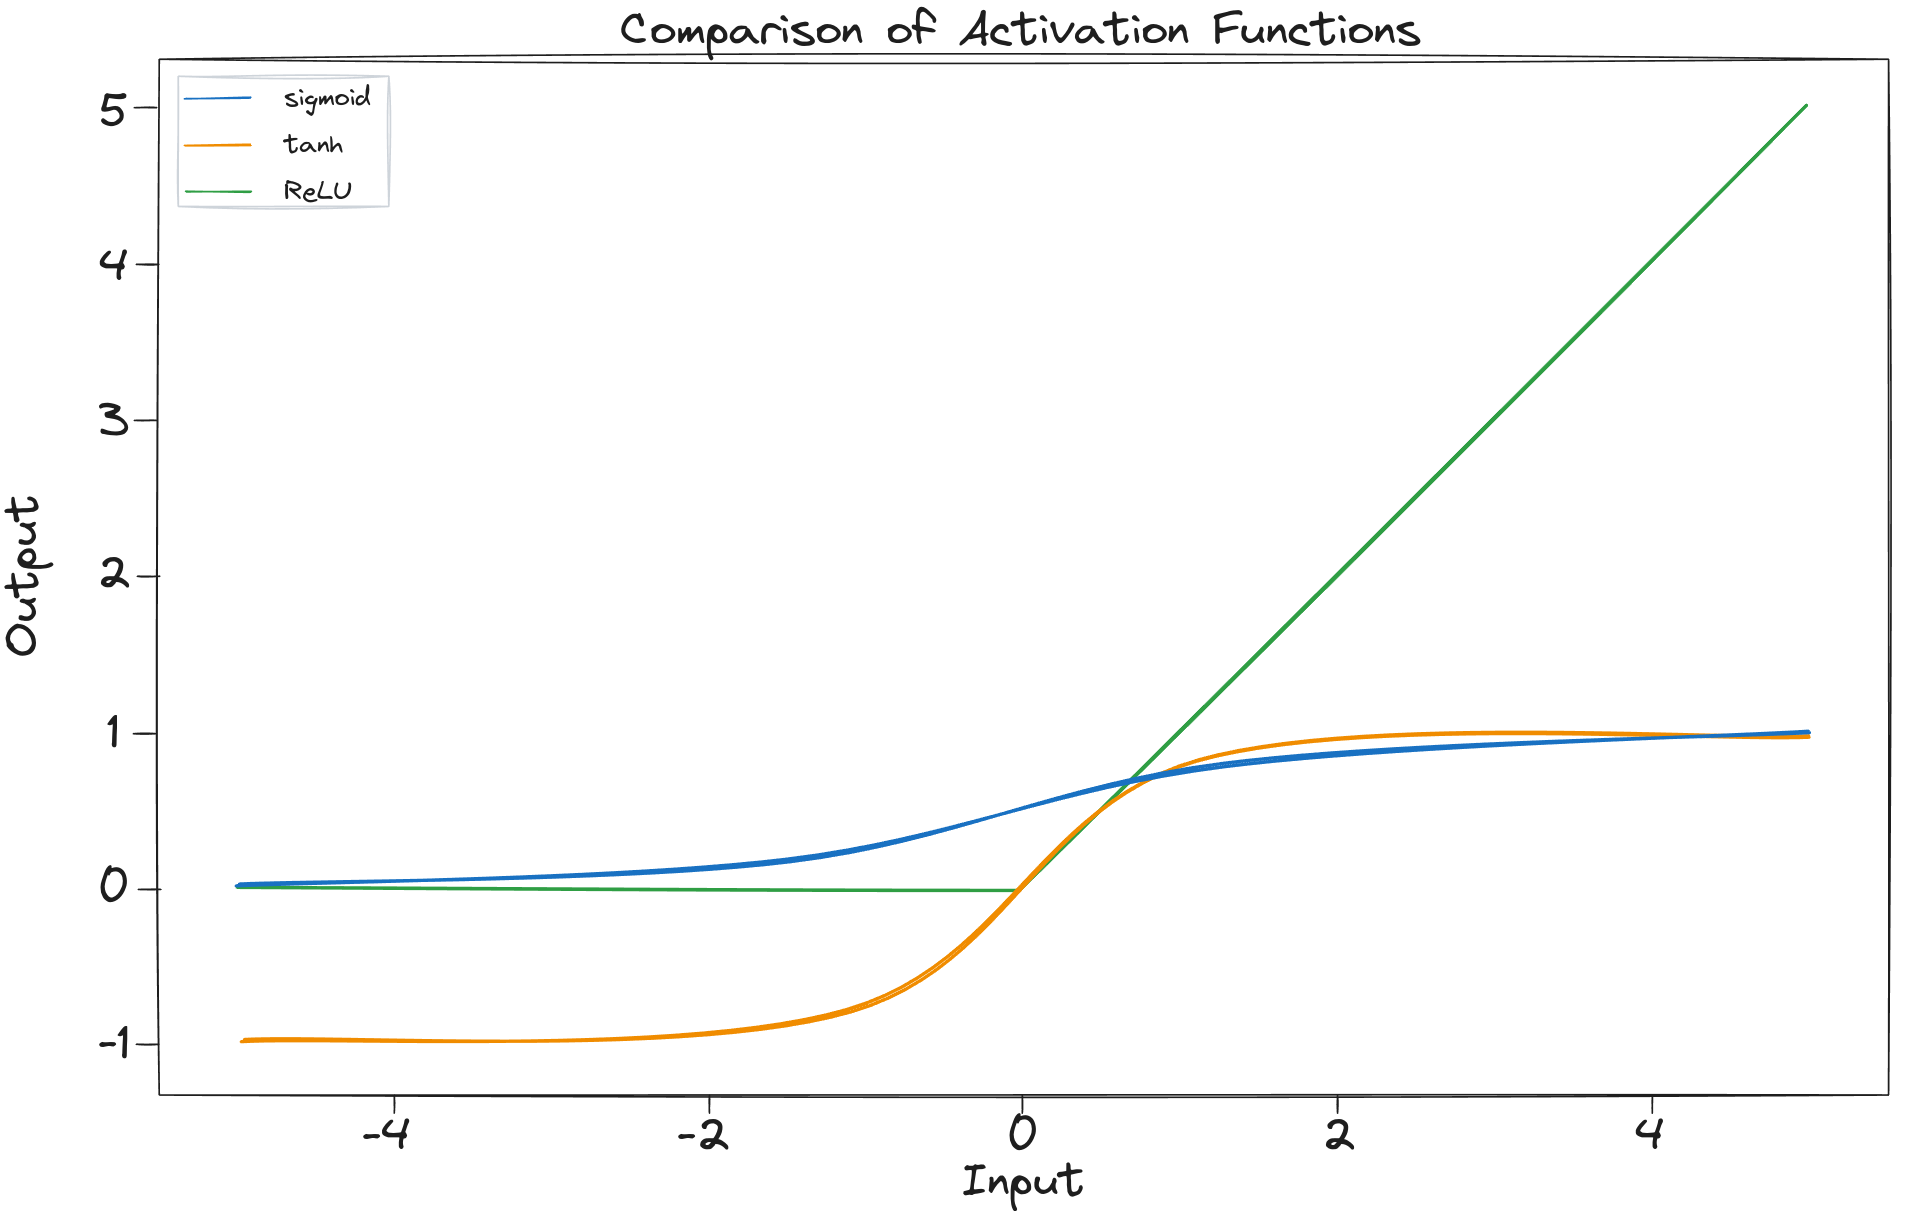
\includegraphics[width=\textwidth,height=6cm,keepaspectratio=true]{activation.png}
    \caption{
        \it{Visualization of the sigmoid, tanh and ReLU activation function outputs.}
    }
    \label{fig:activation}
\end{figure}

The outputs produced by these activation functions exhibit non-linearity, signifying that the input parameter does not linearly determine the output value, as evident from Figure \ref{fig:activation}. This concept holds significance in neural networks, enabling them to learn non-linear systems \cite{doi:10.1080/00207179008934126}. While several activation functions are commonly employed, ReLU has gained prominence in deep learning due to its demonstrated efficacy in enhancing the performance of numerous neural networks \cite{lipton2015critical}. Typically, the same activation function is applied across all neurons, except for those in the output layer.

The choice of activation function for the output layer hinges on the specific task assigned to the neural network. In regression-based tasks, a linear activation function is employed to obtain the summed weighted output of the preceding neurons. Conversely, for classification problems involving \(k\) output neurons, a softmax function is often utilized. The softmax function is defined as:

\begin{equation}
    \hat{y} = \frac{e^{a_k}}{\sum_{j=1}^J e^{a_j}}
\end{equation}

\noindent and ensures that all neuron outputs sum to one on the output layer \cite{lipton2015critical}.

\subsection{Recurrent Neural Networks}
\label{sec:rnn}

Recurrent Neural Networks (RNNs) are specialized neural networks designed for processing sequential data. They operate by incorporating iterations that retain past states, enabling the network to leverage previous inputs as context for the current input \cite{schmidt2019recurrent}. Text serves as a prime example of sequential data, where individual words can be viewed as singular data points within the sequence. Consequently, RNNs can effectively process textual input by utilizing preceding words to predict the subsequent ones. Figure 5 provides an illustration of a basic RNN architecture.


\begin{figure}[H]
    \centering
    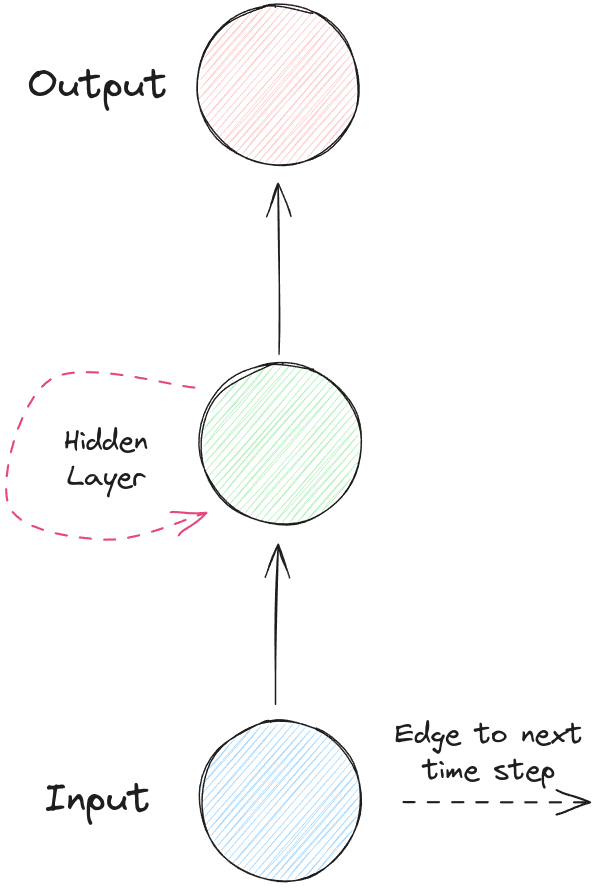
\includegraphics[width=\textwidth,height=6cm,keepaspectratio=true]{rnn.png}
    \caption{
        \it{Visualization of an RNN with one input neuron, one hidden neuron and
            one output neuron \cite{lipton2015critical}.}
    }
    \label{fig:rnn}
\end{figure}

The neuron on the hidden layer stores the hidden state, as visualized by the dashed
line. The activation of the hidden state can be defined as

\begin{equation}
    H_t = \phi_h(X_tW_{xh} + H_{t-1}W_{hh} + b_h)
\end{equation}

where \(H_t\) is the hidden state at time step \(t\), \(\phi_t\) is the activation function of the neuron, \(X_t\) is the neuron input at time step \(t\), \(W_{xh}\) is a weight matrix, \(W_{hh}\) is the weight matrix of the hidden state and \(b_h\) is bias \cite{schmidt2019recurrent}.

RNNs are trained utilizing the backpropagation through time (BPTT) algorithm, which is an adaptation of the standard backpropagation algorithm tailored for networks with a sequential order of computations. In this setup, the output at time step \(t\) depends on the states from preceding steps \cite{58337}. During training, the forward pass computes through all time steps, and the resultant loss is utilized to update the parameters across all time steps. One way to conceptualize this process is by envisioning an unrolled RNN, where the recurrent loops are eliminated, resulting in a network structure akin to a feedforward neural network. However, due to the nature of the hidden state dynamics, RNNs are notorious for encountering gradient-related issues during training. As illustrated in Figure \ref{fig:gradient}, if the weight associated with the dotted line is less than one, future values may decrease exponentially \cite{lipton2015critical}. Conversely, weights that start to grow can lead to the exploding gradient problem \cite{schmidt2019recurrent}. When gradients become too small or too large, it can impede the training process of the model.


\begin{figure}[H]
    \centering
    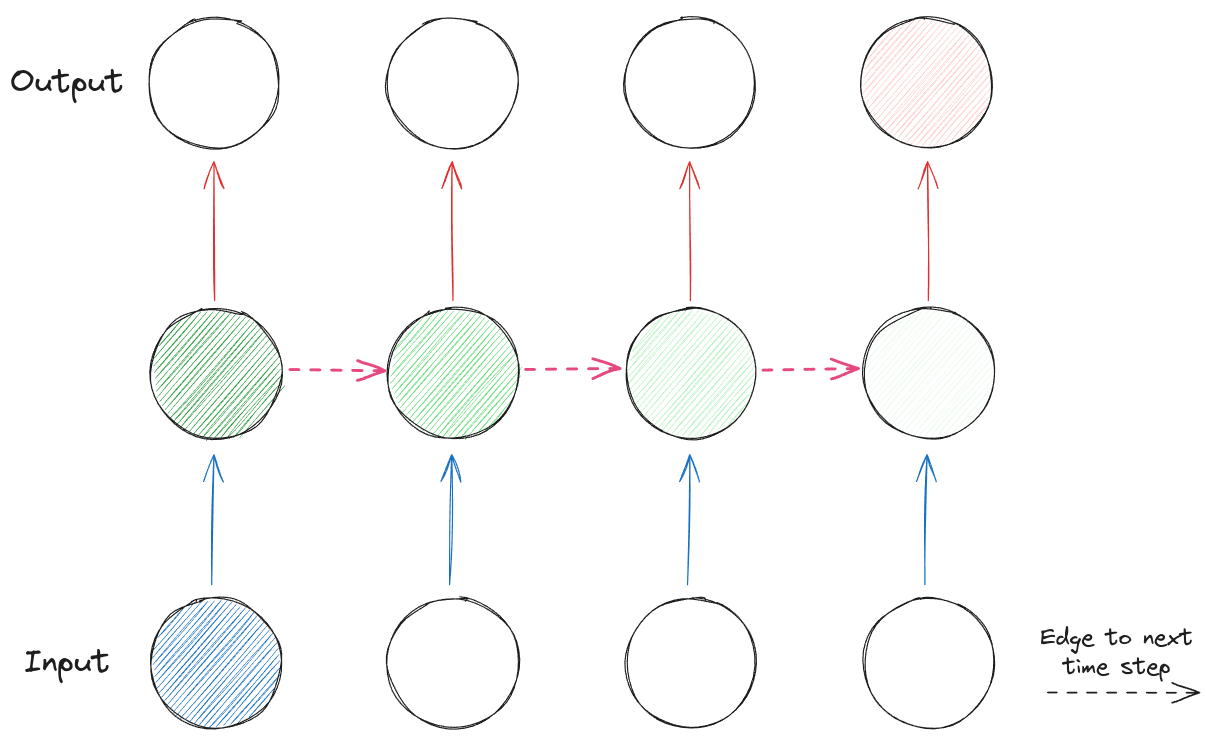
\includegraphics[width=\textwidth,height=6cm,keepaspectratio=true]{gradient.png}
    \caption{
        \it{Visualization of the vanishing gradient problem, which is indicated by the
            hidden neuron color fading away \cite{lipton2015critical}.}
    }
    \label{fig:gradient}
\end{figure}

Despite offering a robust framework for sequential learning, RNNs are hindered by significant limitations arising from the aforementioned issues. One critical limitation stems from the gradient problem encountered during training, which can constrain the effective handling of lengthy sequences. Consequently, RNNs may struggle to capture dependencies between inputs across extended sequences. To address these challenges, numerous techniques and alternative architectures have been proposed. Among these, the Long Short-Term Memory (LSTM) architecture stands out as one of the most prominent examples, and its discussion follows.

\subsection{Long Short-Term Memory}

The Long Short-Term Memory (LSTM) \cite{10.1162/neco.1997.9.8.1735} architecture addresses the gradient-related challenges inherent in RNNs by incorporating constant error, memory cells, and gate units. This design enables the network to effectively handle sequences spanning over 1000 time steps. The memory cells employ three gate units: an input gate \(I_t\), an output gate \(O_t\), and a forget gate \(F_t\), which regulate the flow of information. Specifically, the input gate facilitates the addition of information to the memory cell, the output gate facilitates information retrieval from the cell, and the forget gate facilitates cell resetting \cite{schmidt2019recurrent}. Moreover, the memory cells possess an internal state with a self-connected recurrent edge featuring a constant weight, ensuring consistent error propagation across time steps and mitigating previously discussed gradient-related issues \cite{lipton2015critical}. Additionally, a candidate memory cell \(\tilde{C}\), utilized for proposing new information, is integrated with the old memory content \(C_{t-1}\) through the gates to govern the preservation of old memory in the new memory \(C_t\) \cite{schmidt2019recurrent}. Figure \ref{fig:lstm} illustrates the complete architecture of the LSTM memory cell.

\begin{figure}[H]
    \centering
    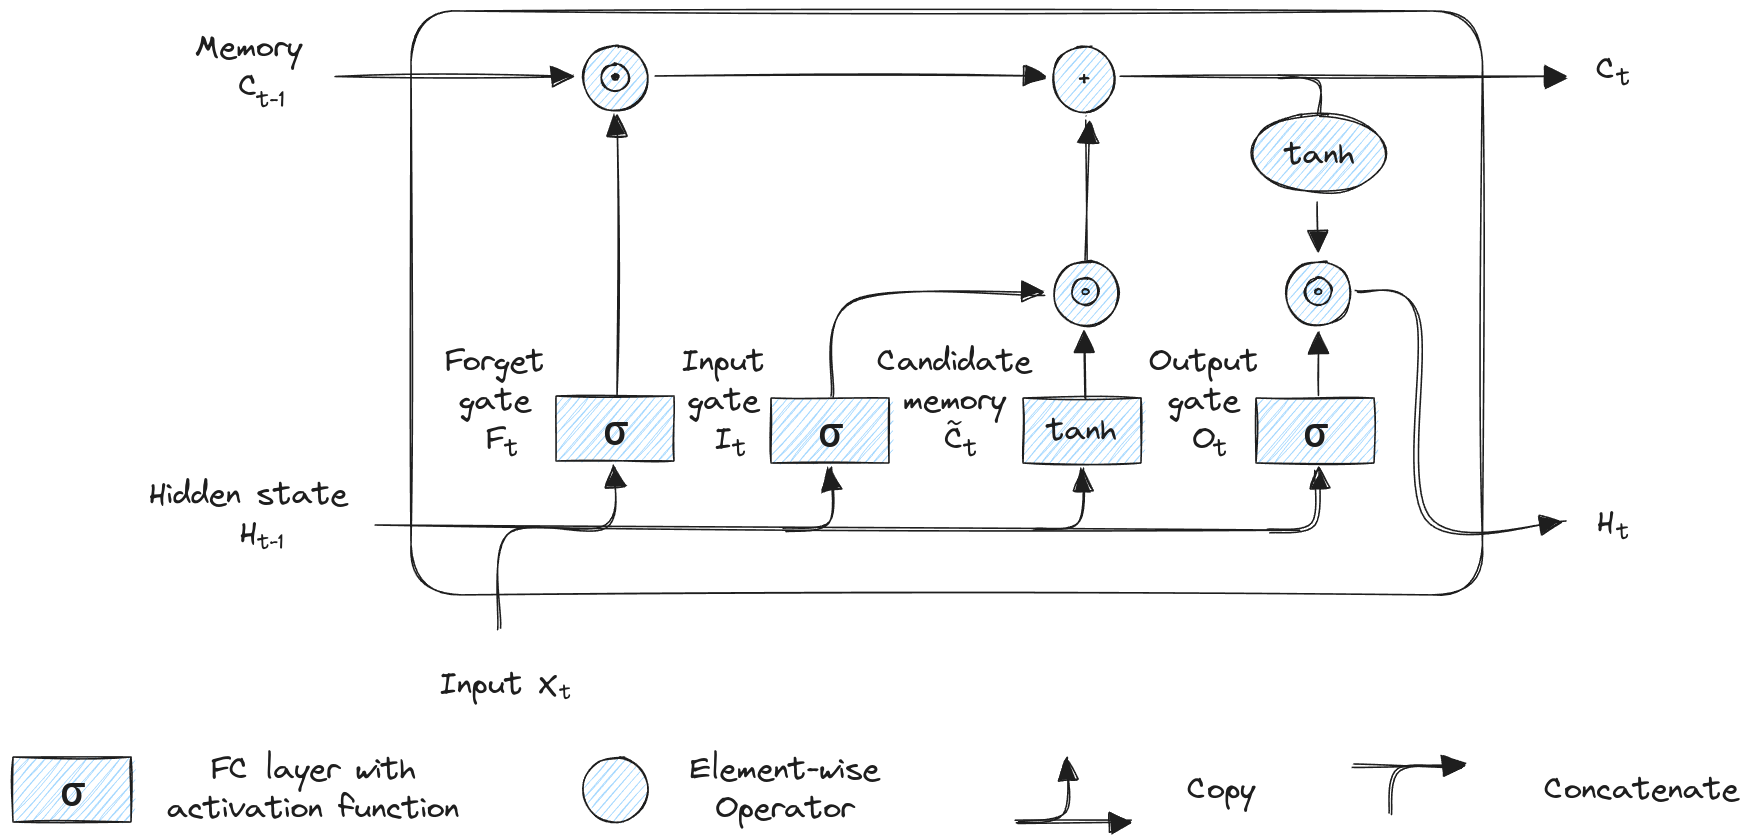
\includegraphics[width=\textwidth,height=6cm,keepaspectratio=true]{lstm.png}
    \caption{
        \it{Visualization of an LSTM memory cell \cite{schmidt2019recurrent}.}
    }
    \label{fig:lstm}
\end{figure}

Although the LSTM architecture enhances performance compared to the RNN architecture discussed in \autoref{sec:rnn}, it still possesses limitations. Like the RNN architecture, models utilizing LSTM must process the previous time step before computing the next, rendering them computationally intensive and impeding parallelization. Additionally, LSTM typically lacks an explicit attention mechanism and tends to prioritize the most recent words. These constraints are addressed by the Transformer model, which will be introduced next.


\clearpage

\section{Large language models (LLMS)}

Large language models utilize deep neural networks to generate human-like language output by learning patterns from extensive text data. These models excel at various NLP tasks, including language generation, machine translation, question answering, and sentiment analysis.

The advent of transformer-based architectures, exemplified by GPT (Generative Pre-trained Transformer) and BERT (Bidirectional Encoder Representations from Transformers), marks a recent breakthrough in large language models. These models undergo pre-training on vast datasets, allowing them to learn from massive amounts of data. Subsequently, they can be fine-tuned for specific tasks.

In recent years, large language models like GPT-3 and the more recent GPT-4 have witnessed a significant enhancement in performance and capabilities, achieving remarkable results across a diverse array of benchmarks.

LLMs use various NLP tasks to achieve their goals. For example, tokenization can be
used for pricing the LLM usage when used tokens are counted \cite{openai:tokens}, the models summarize texts, answer questions, etc. Different applications that use NLP are search engines,language translation services, chatbots, text summarization, and question-answering.
While LLMs can incorporate all these tasks and applications, their performance may differ
from those designed for a specific task.

\begin{figure}[H]
    \centering
    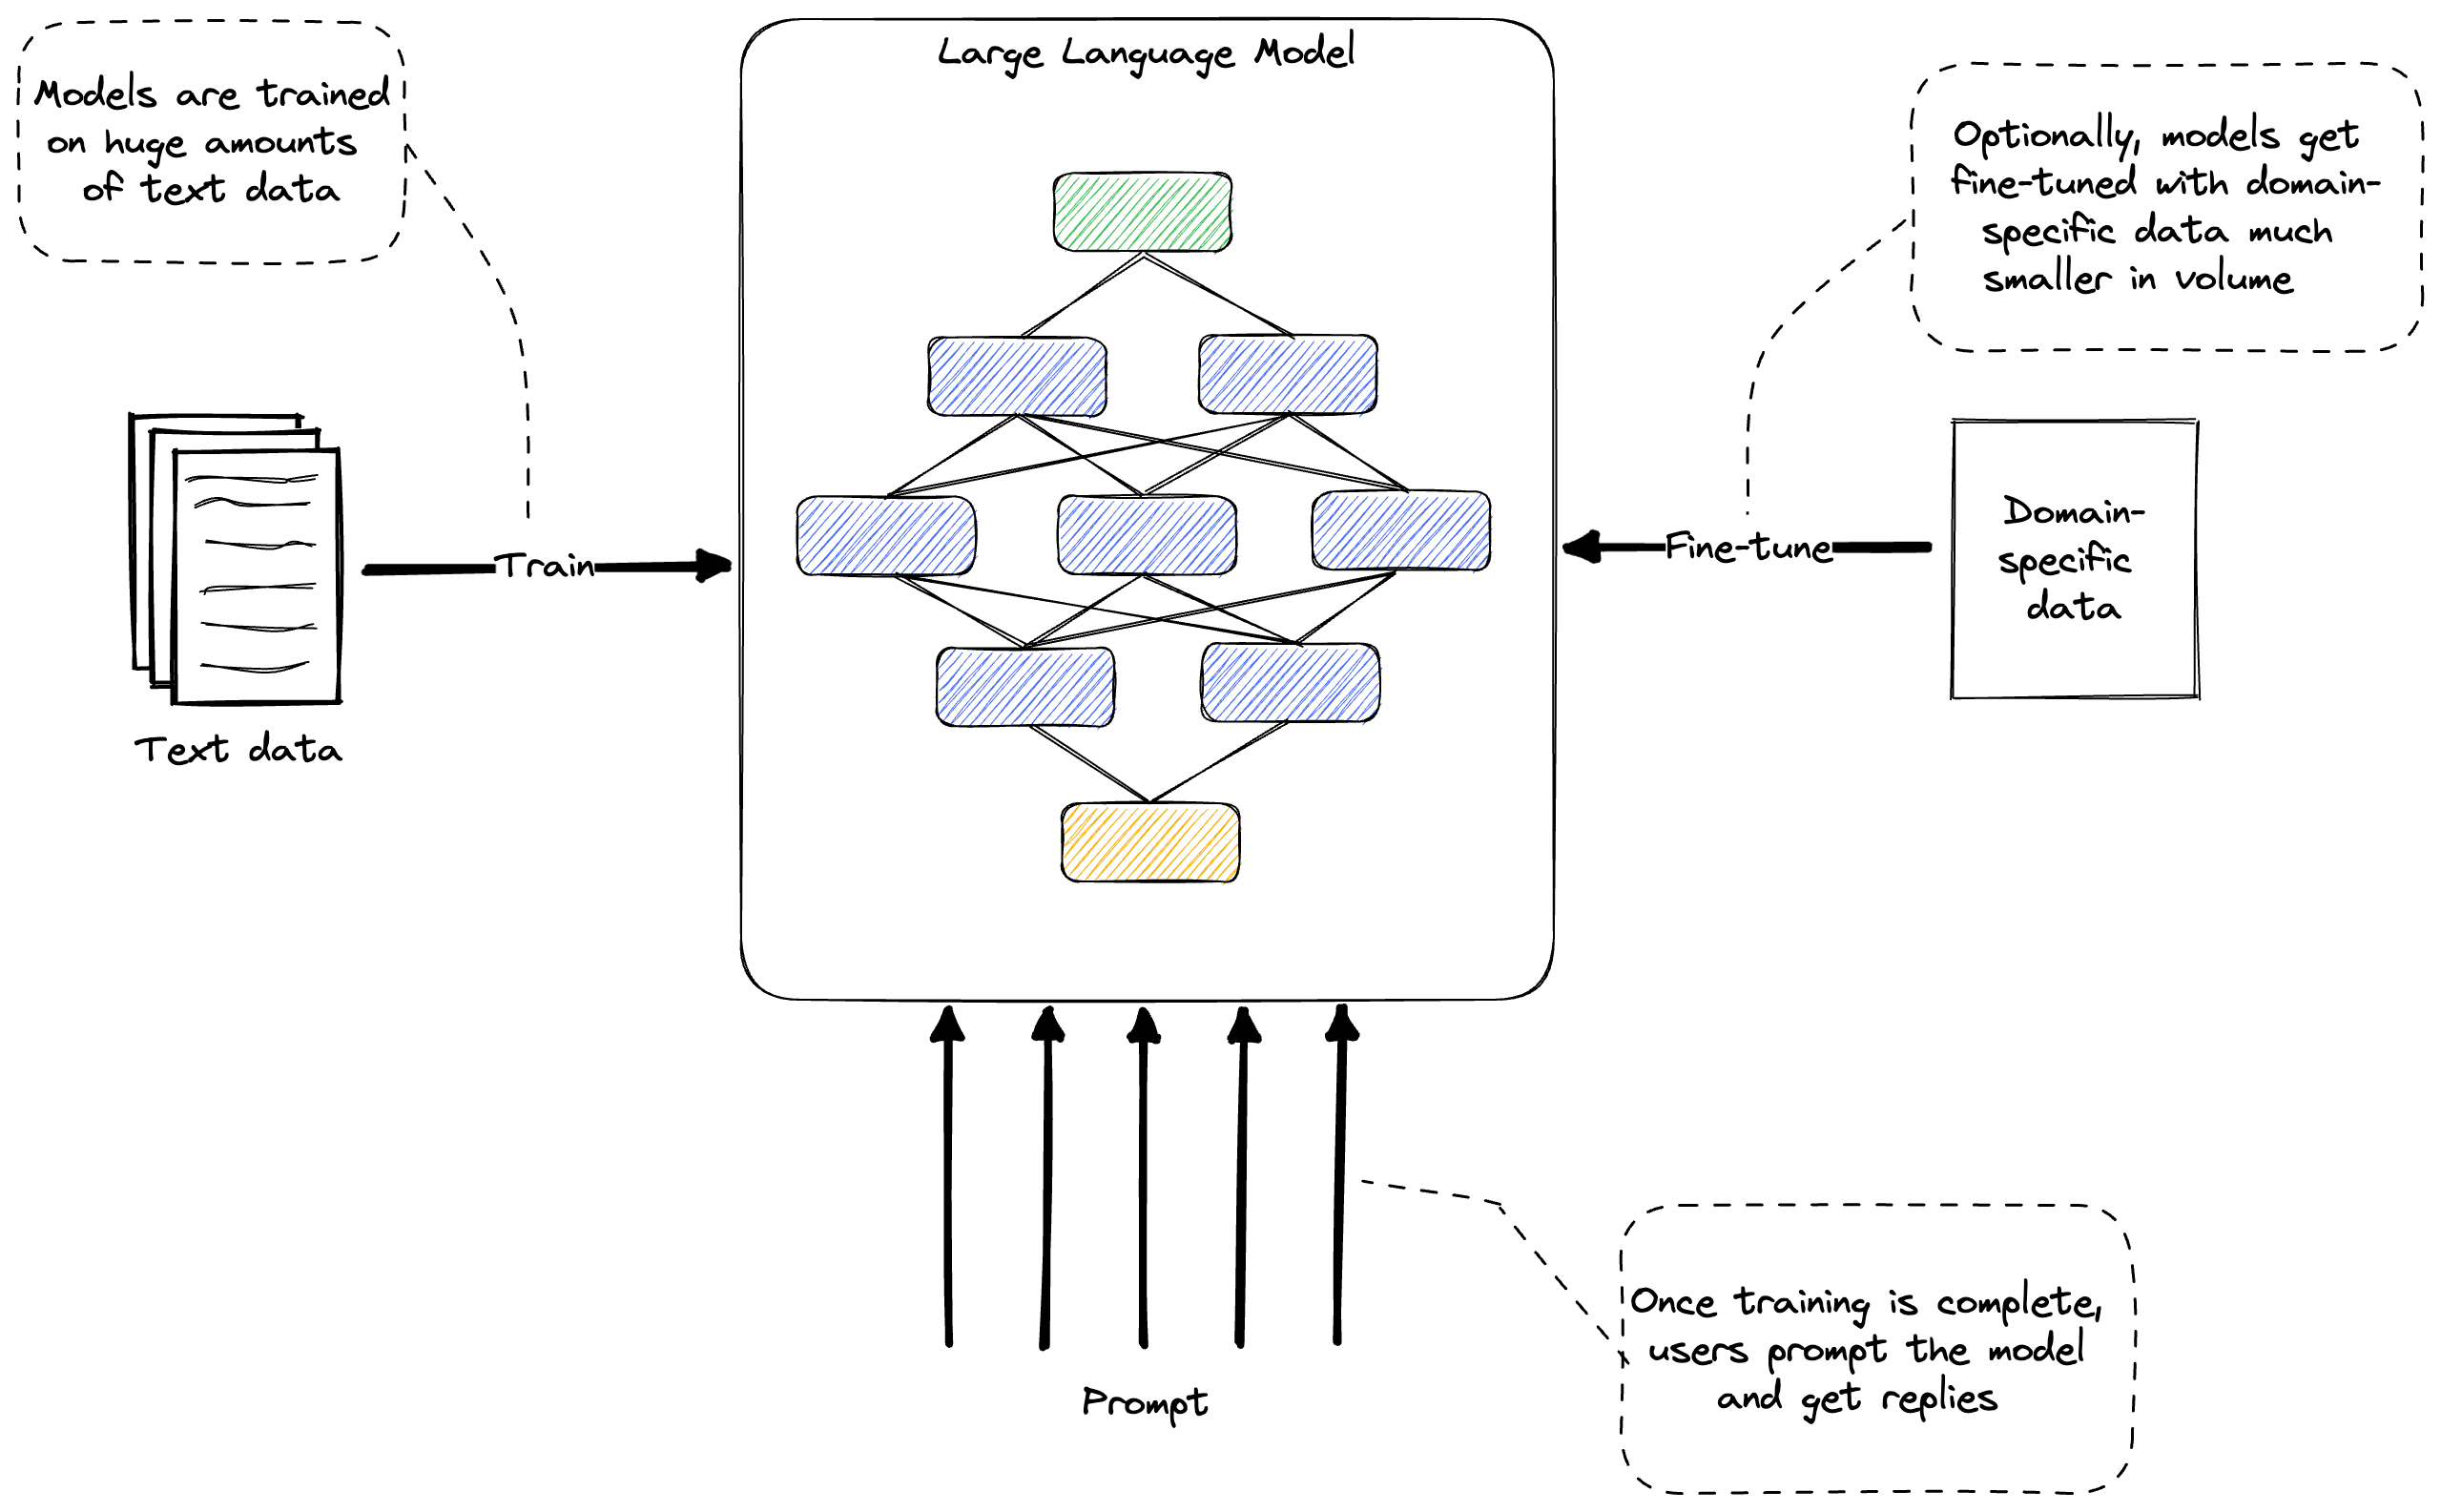
\includegraphics[width=\textwidth,height=6cm,keepaspectratio=true]{llms.png}
    \caption{
        \it{Training, fine tuning, and prompting.}
    }
\end{figure}

\subsection{History of Large Language Models}

Over the years, the development of LLMs has been propelled by advancements in NLP, machine learning, and computing resources. This section offers a comprehensive overview of the significant milestones and breakthroughs that have shaped the evolution of LLMs.

\subsubsection*{Pre-Transformer Era}

\begin{enumerate}
    \item \textbf{Eliza (1964-1966):} One of the earliest NLP programs, Eliza was a simple chatbot developed by Joseph Weizenbaum, designed to mimic a Rogerian psychotherapist. It used pattern matching and substitution to generate responses, laying the foundation for future conversational AI systems.
    \item \textbf{Statistical language models (1980s-2000s):} Statistical language models, such as n-grams, were developed to predict the probability of a word in a sequence based on the preceding words. These models were widely used in tasks like speech recognition and machine translation but struggled with capturing long-range dependencies in text.
    \item \textbf{Neural language models (2003-2013):} Neural language models, such as feedforward and recurrent neural networks (RNNs), emerged as an alternative to statistical models. Bengio et al. (2003) introduced a feedforward neural network for language modeling, while Mikolov et al. (2010) popularized RNN-based models with the release of the RNNLM toolkit.
    \item \textbf{Long Short-Term Memory (LSTM) models (1997-2014):} Hochreiter and Schmidhuber (1997) introduced LSTMs as a solution to the vanishing gradient problem faced by RNNs. LSTMs were later used in sequence-to-sequence models for tasks like machine translation (Sutskever et al., 2014) and formed the basis for several LLMs.
\end{enumerate}

\subsubsection*{Transformer Era}

\begin{enumerate}
    \item \textbf{Attention is All You Need (2017) \cite{vaswani2023attention}:} Vaswani et al. introduced the transformer architecture, which replaced the recurrent layers in traditional models with self-attention mechanisms. This breakthrough enabled the development of more powerful and efficient LLMs, laying the foundation for GPT, BERT, and T5.
    \item \textbf{GPT (2018) \cite{openai:gpt}:} OpenAI released the Generative Pre-trained Transformer (GPT), a unidirectional transformer model pre-trained on a large corpus of text. GPT showcased impressive language generation capabilities and marked the beginning of a new era of LLMs.
    \item \textbf{BERT (2018) \cite{devlin2019bert}:} Google introduced the Bidirectional Encoder Representations from Transformers (BERT) model, which used a masked language modeling objective to enable bidirectional context representation. BERT achieved state-of-the-art performance on numerous NLP tasks, revolutionizing the field.
    \item \textbf{GPT-2 (2019) \cite{radford2019language}} OpenAI released GPT-2, a significantly larger and more powerful version of the original GPT. GPT-2 demonstrated impressive text generation capabilities, generating coherent and contextually relevant text with minimal prompting.
    \item \textbf{T5 (2019) \cite{raffel2023exploring}:} Google's Text-to-Text Transfer Transformer (T5) adopted a unified text-to-text framework for pre-training and fine-tuning, allowing it to be used for various NLP tasks by simply rephrasing the input and output as text. T5 demonstrated state-of-the-art performance across multiple benchmarks.
    \item \textbf{GPT-3 (2020) \cite{brown2020language}:} OpenAI unveiled GPT-3, an even larger and more advanced version of the GPT series, with 175 billion parameters. GPT-3's performance on various NLP tasks with minimal fine-tuning raised questions about the capabilities and potential risks associated with LLMs.
\end{enumerate}

The history of large language models is marked by continuous innovation and progress in the field of natural language processing. As we move forward, LLMs are expected to grow in size, capability, and efficiency, enabling more complex and human-like language understanding and generation. However, the development of these models also brings forth ethical and practical challenges that must be addressed, such as biases, misuse, and computational resource requirements. It is essential for researchers and practitioners to balance the potential benefits of LLMs with their limitations and risks, fostering responsible development and use of these powerful tools.